\documentclass[12pt]{article}
\usepackage[utf8]{inputenc}
\usepackage[russian]{babel}
\usepackage[margin=1.5in,left=1cm,right=1cm, top=2cm,bottom=2cm,bindingoffset=0cm]{geometry}
\usepackage{graphicx}
\usepackage{color}
\usepackage{amssymb}
\usepackage{minted}
\usepackage{hyperref}
\usepackage{amsmath}
\usepackage{fancyhdr}



\title{Title}
\author{Амеличев Константин, ПМИ 191.}
\date{Date}

\newcommand{\problem}[2]{

\section {Задача #1}
\textbf {Постановка задачи.} {#2}

\textbf {Решение.}
}

\newcommand{\limit}[2]{\displaystyle \lim_{#1 \to #2}}

\newcommand{\rangesum}[2]{\displaystyle \sum_{#1}^{#2}}

\newcommand{\mintedparams}{
% frame=lines
% framesep=2mm,
% baselinestretch=1.2,
% bgcolor=LightGray    
}

\pagestyle{fancy}
\fancyhf{}
\fancyhead[LE,RO]{Амеличев Константин, ПМИ 191, @kik0s, \href{http://github.com/kik0s}{\textcolor{blue}{github}}, \href{http://codeforces.com/profile/kikos}{\textcolor{blue}{codeforces}}, \href{http://vk.com/i_tried_to_name_myself_kikos}{\textcolor{blue}{vk}}}
\fancyhead[RE,LO]{Лекция АиСД 16.01}

\begin{document}

\paragraph{Запросы на деревьях.} Будем обсуждать две задачи: \textbf{LCA} и \textbf{LA}. 

Постановка задачи $LCA$: даются запросы на вычисления наименьшего общего предка двух вершин $v,\,u$. То есть, ответ на запрос~--- это вершина наибольшей глубины такая, что она является предком и $v$, и $u$.

Постановка задачи $LA$: даются запросы на вычисления предка вершины $v$ на глубине $k$.

\paragraph{Двоичные подъемы.} Для каждой вершины преподсчитаем $p_{v,i}$, которая будет хранить информацию о том, какая вершина является $2^i$-ым предком вершины $v$. Насчитать их можно с помощью обхода дерева за $O(n \log n)$.

Решение задачи $LA$ с помощью двоичных подъемов тогда будет таким: разложим число $k$ на степени двойки, и сделаем соответствующие <<прыжки>>: $v \rightarrow p_{v,i_1} \rightarrow p_{p_{v,i_1}, i_2} \rightarrow \ldots$.

Решение задачи $LCA$ будет таким: сначала мы выровняем вершины по глубине. Иначе говоря, решим задачу $LA$, чтобы после ее решения вершины запроса имели одинаковую глубину (при этом мы хотим двигать только более глубокую вершину). Теперь, когда вершины на одной глубине (и если не совпали!), мы будем двигаться по степеням двойки от больших к меньшим таким образом: Если $LA_{2^i}$ наших вершин не совпали, то тогда поднимем вершины запроса на $2^i$. Такой процедурой мы найдем таких предков вершин $u$ и $v$, которые не совпадают, находятся на одной глубине, и при этом имеют общего предка. Этот предок и будет ответом на задачу.

Решение с двоичными подъемами работает за $O(n \log n)$ преподсчета и $O(\log n)$ на запрос для обеих задач.

\paragraph{Offline.} Решить $LA$ в оффлайн можно обходом в глубину с поддержкой стека за $O(n + q)$. Решение $LCA$ в оффлайн можно сделать с помощью алгоритма Тарьяна с СНМом (просто как факт) за $O((n + q) \alpha)$

\paragraph{Эйлеров обход.} Мысленно превратим каждое ребро в два ребра, одно из которых ориентировано вверх, а другое вниз. Тогда в таком графе можно сделать обход по типу Эйлерова~--- каждое ребро пройдем ровно один раз. Будем выписывать вершину $v$ каждый раз, когда проходим по ребру из $v$.

\begin{center}
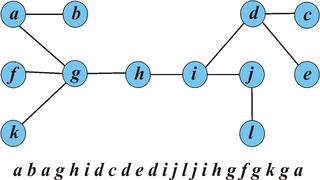
\includegraphics{pictures/euler_path_on_tree.png}
\end{center}

Строго говоря, обход можно делать не из корня, а просто потом сделать циклический сдвиг, но обычно все запускают обход из корня и не парятся.

Важное свойство~--- подотрезок нашего обхода является путем. При этом путь между $u$ и $v$ в эйлеровом обходе содержит $LCA(u,\,v)$ (потому что путь из $u$ в $v$ точно проходит через $LCA(u,\,v)$), а еще не содержит предка $LCA(u,\,v)$ (потому что по ребру в него проход был дважды, и если мы посетим его после $lca$, то мы уже не могли спуститься обратно). То есть, $LCA$ будет самой высокой вершиной на подотрезке обхода между $u$ и $v$. Это является сведением к задаче $RMQ$. Тогда с помощью sparse table можно получить решение за $O(n \log n + q)$.

$LA$ тоже можно решать с помощью эйлерова обхода, делая спуск по дереву отрезков с поиском первой вершины на высоте хотя бы $k$.

\paragraph{Метод четырех русских.} Пушка, которая решит нам $LCA$ за $O(n + q)$. Мы разобьем задачи на большие и маленькие. Нам не обязательно решать маленькие задачи при их появлении, если мы можем заранее решить все возможные маленькие задачи.

\paragraph{$RMQ \pm 1$.} Заметим, что наше $RMQ$ при поиске $LCA$ обладала тем свойством, что $a_i = a_{i - 1} \pm 1,\ a_i \neq a_{i - 1}$. Разобьем массив на блоки размера $k$, в каждом блоке посчитаем максимум и получим массив $b_1,\ \ldots\ ,\ b_{\frac{2n}{k}}$. Насчитаем на нем разреженные таблицы. Также в блоке насчитаем префиксные и суффиксные максимумы. Теперь мы умеем за $O(1)$ отвечать на все запросы, кроме тех, которые полностью лежат в одном блоке.

Для решения такой задачи мы посчитаем все возможные последовательности из $\pm 1$ длины $k$, там возьмем все подотрезки, и для них за линию решим. То есть за $O(2^k \cdot k^3)$. Можно, наверное, и лучше, но нам пофиг.

Теперь положим $k = \lceil \frac{\log n}{2} \rceil$. Тогда маленькая задача решится за $O(\sqrt{n} \cdot \log^3 n)$. А для большой задачи преподсчет будет работать за $O(\frac{n}{k} \log n) = O(n)$. Таким образом, задача решена за $O(n + q)$.

Решение произвольного $RMQ$ делается с помощью $RMQ \rightarrow LCA \rightarrow RMQ \pm 1$. Первый переход делается с помощью построения ДД на массиве с помощью стека. Тогда $RMQ$ на отрезке это $LCA$ для соответствующих вершин.

\paragraph{Ladder decomposition.} Предложим другое решение задачи $LA$. Разобьем дерево на пути таким образом: возьмем самую высокую вершину, которая еще не покрыта путями, и возьмем из нее самый глубокий путь вниз. Также насчитаем двоичные подъемы. Такое можно решить за $O(n \log n)$. Каждый путь выпишем явно.

После этого мы мысленно удвоим все пути. Возьмем и выпишем еще столько же вершин вверх для каждого пути. Общая память все еще линейна.

Теперь пусть нам надо сделать подъем на $k$. Найдем наибольшее $i$ такое, что $2^i \le k$, сделаем такой прыжок. После чего мы оказываемся в вершине, самый глубокий путь из которой вниз был по длине не меньше, чем $2^i$. Это значит, что ответ на задачу хранится в выписанном пути для этой вершины и его можно найти за $O(1)$.

\end{document}
